\begin{XeClass}{UmaskParser}
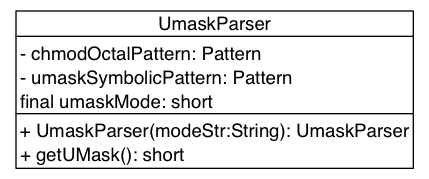
\includegraphics[width=\textwidth]{cdig/UmaskParser.png}
     
 解析String中提供的八进制或符号形式的umask模式, 并返回short型整数(以八进制形式).
 Umask形式与标准形式略有不同, 它们不能指定"sticky bit"(粘滞位, 用于限制用户在公共目录中修改他人文件),
 也不能指定"special execute"(X, 拥有该标记的目录下的所有文件被无条件赋予可执行权限).

    \begin{XeMethod}{\XePublic}{short}{getUMask}
         
 仅用于创建文件/目录. 符号形式的umask被用于描述"相对权限模式", 使用'+'或'-'来对
 原有的权限模式进行复位或置位.
 对八进制形式的umask而言, 指定的模式位通过创建时的模式给出.
 For octal umask, the specified bits are set in the file mode creation mask.

    \end{XeMethod}

\end{XeClass}
